\section{Introduction}
\label{Chapter:Introduction}
{
    Islamic calligraphy is an art having a history that dates back to the seventh century \cite{bib01, bib02}. It has witnessed many evolutionary stages \cite{bib02, bib03} and has been used by artists speaking several different languages \cite{bib04} and sharing uncommon biographies \cite{bib05,bib06,bib07,bib08}. Unfortunately though, the industrial age and the advent of technology has not spared this beautiful art when it claims to provide better alternatives for almost everything related to human beings. Discovery of new facets of calligraphy aside, with the prevalence of modern technologies and resulting lack of expertise in this domain, the very existence of Islamic calligraphy now faces a serious threat. Public buildings and infrastructure that once used to be a showcase for the most laudable artists of the time have turned in-to museums; awaiting to be wiped away slowly with each round of the monsoon and every splash of the ocean’s waves. Such a site is shown in Figure \ref{Fig:BegumShahi}


    \begin{figure}
      \centering
      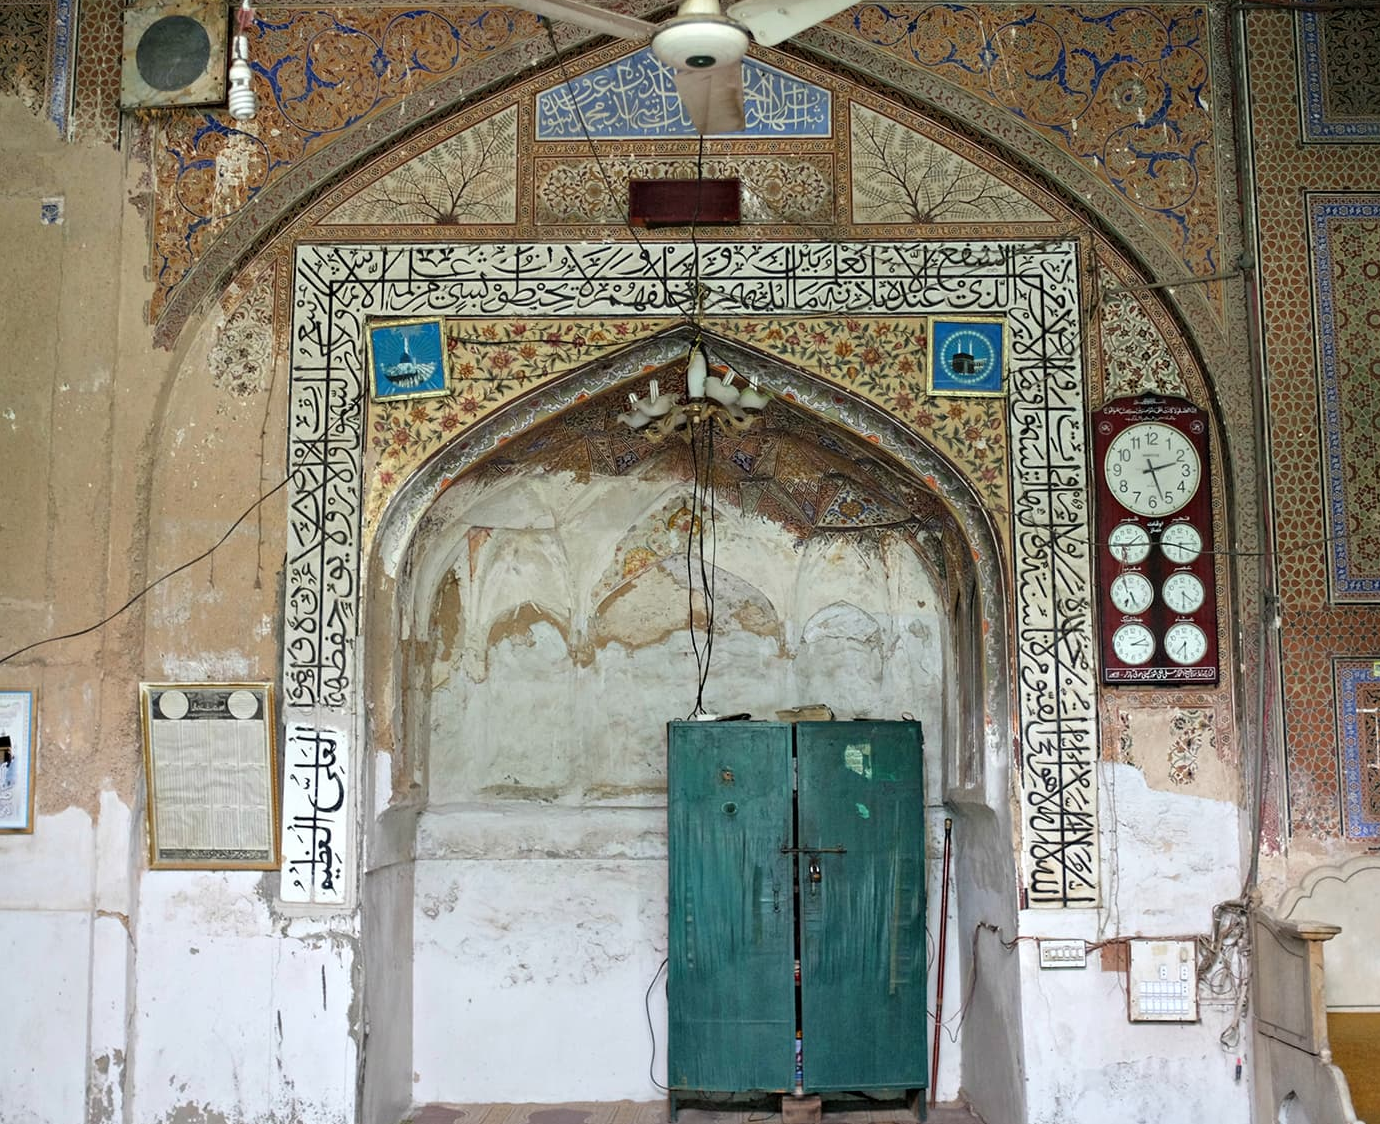
\includegraphics[width=0.9\textwidth]{../Images/BegumShahi.pdf}
      \caption{A photo of a wall inside Mariyam Zamani Mosque (also known as Begum Shahi Masjid) Lahore. Some of the calligraphy has been reconstructed (highlighted in red) using conventional techniques and can easily be recognised because it looks different than the rest.
      } \label{Fig:BegumShahi}
    \end{figure}


    Potentially, we can use robotic dexterity to help us in this domain. Industrial robots have already been used outside the industry to do unorthodox tasks \cite{bib09, bib10,bib11,bib12} and they can surely uplift this art as well. At the very least, they can be employed in restoration and replication of existing calligraphy work \cite{bib13}. In other words, they can be used as printers, or rather one may say, “painters” that give an extra hand to the calligraphy artists to open up a new dimension of art that can not only revamp the existing calligraphy sites but also create new ones.

    Mechanized/robotic drawing of the Islamic calligraphy scripts requires not just the ink-mark information but also the information about the tool movement \cite{bib03}. Compared to the industrial color printers that mostly print on flat surface, or rolled surfaces at worst, using a flexible broad edge brush to draw on a possibly un-even curved surfaces situated in narrow spaces, makes the job relatively more complex. A robot needs to take special care about the tool orientation and downwards force of the tool as well.

    Since an industrial robotic arm can accurately maneuver paths in three dimensional space with controlled speed and downward force, the main problem is limited to two parts. First, discover a method that can not only trace existing specimens but can also allow modifying and creating new ones. Second, discovering a method to extract machine data from the graphics data.
    

    This research proposes one solution to answer both of these questions: unify the graphics data with machine data. Conventionally, the kind of data used by the computer to render and print graphics on the screen or on paper fundamentally differs from the data needed by a machine that uses a mechanical end effector to produce output. We propose a rather simple innovation in the conventional bezier splines which enables them to mimic the ink-mark of broad-edge tools and can directly generate machine movement data. We name them ``Rotating/twisting Bezier Spline Curves'', or simply, ``Twisting Bezier Splines''.

    Ink-mark in most of islamic calligraphy scripts is usually a result of multiple closely located tool strokes that form up words by overlapping letters. Also, as a result of spin of a broad-edge tool, the width of the strokes continuously vary. No computer algorithm currently exists that can accurately determine the pitch lines of these strokes because of these complexities. It is discussed in following chapters why this pitch line is the key to the generation of machine data for reconstruction of the scripts. The research presented here proposes a human assisted technique to accurately extract these pitch lines in the same fashion as a real artist would be intended. This new method becomes a possibility mainly due to the ``Twisting Bezier Splines''

    The article is divided in $5$ sections. After the introduction, Chapter \ref{Chapter:SplineModelling} presents the working principle and mathematical model of the twisting/rotating bezier splines. In section \ref{Chapter:Performance} we discuss some performance metric and discuss the tests performed to gauge the performance of the twisting bezier splines. Section \ref{Chapter:Simulation} discusses the simulation of a robotic manipulator to verify the results. We finally conclude in Section \ref{Chapter:Conclusion}. The software tools used in this research, the software user manuals, video tutorials and the source codes can be viewed on GitHub \cite{bib20}.
    }